\documentclass{jsarticle}
\usepackage[dvipdfmx]{graphicx}
\usepackage{listings}
\usepackage{afterpage}
\begin{document}
\title{課題10 エッジ抽出}
\author{13EC060 武澤 裕介}
\maketitle
\begin{abstract}
matlabを用いて、エッジの抽出を行う。
\end{abstract}
\section{エッジ抽出}
まず、今回使用する原画像を図1に示す。


\begin{figure}[htbp]
 \begin{center}
  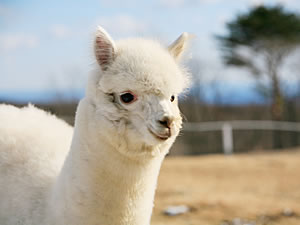
\includegraphics[width=5cm,height=5cm]{a.jpg}
 \end{center}
 \caption{原画像}
\end{figure}

\begin{lstlisting}[basicstyle=\ttfamily\footnotesize, frame=single]
filename = uigetfile('*');
ORG=imread(filename); % 原画像の入力
ORG = rgb2gray(ORG); colormap(gray); colorbar;
imagesc(ORG); axis image; % 画像の表示
pause; % 一時停止
 \end{lstlisting}
を用いてまず入力画像のグレースケール画像を表示させる。

\newpage
\begin{figure}[htbp]
 \begin{center}
  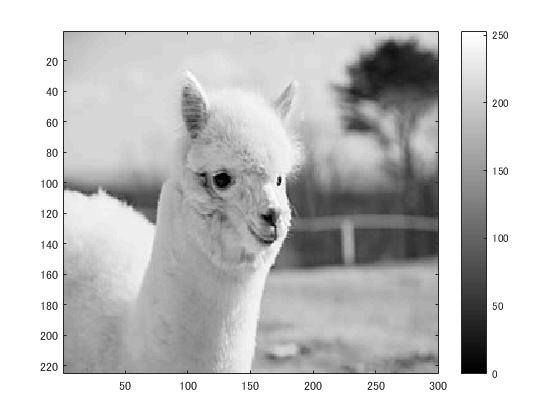
\includegraphics[width=10cm]{8-0.jpg}
 \end{center}
 \caption{グレースケール画像}
\end{figure}

最後に
\begin{lstlisting}[basicstyle=\ttfamily\footnotesize, frame=single]
IMG = edge(ORG,'prewitt'); % エッジ抽出(プレウィット法)
imagesc(IMG); colormap('gray'); colorbar;% 画像表示
pause; % 一時停止

IMG = edge(ORG,'sobel'); % エッジ抽出(ソベル法)
imagesc(IMG); colormap('gray'); colorbar;% 画像表示
pause; % 一時停止

IMG = edge(ORG,'canny'); % エッジ抽出(キャニー法)
imagesc(IMG); colormap('gray'); colorbar;% 画像表示
pause; % 一時停止
 \end{lstlisting}
を用いてエッジの抽出を様々な方法にて行う

\newpage
\begin{figure}[htbp]
 \begin{center}
  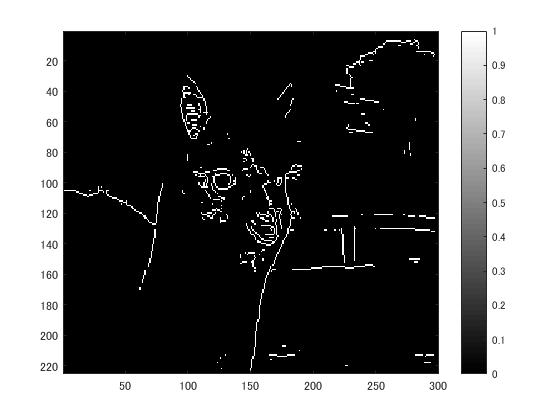
\includegraphics[width=10cm]{8-1.jpg}
 \end{center}
 \caption{エッジの抽出(プレウィット法)}
\end{figure}

\newpage
\begin{figure}[htbp]
 \begin{center}
  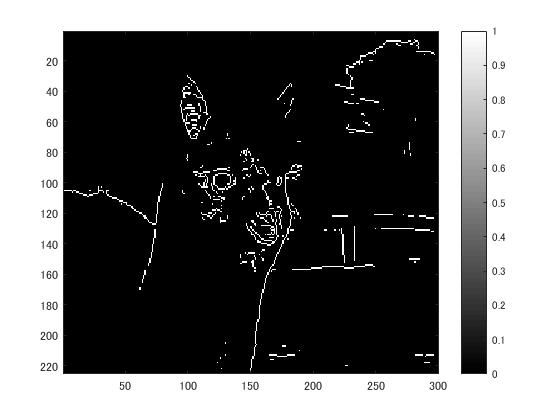
\includegraphics[width=10cm]{8-2.jpg}
 \end{center}
 \caption{エッジの抽出(ソベル法)}
\end{figure}

\newpage
\begin{figure}[htbp]
 \begin{center}
  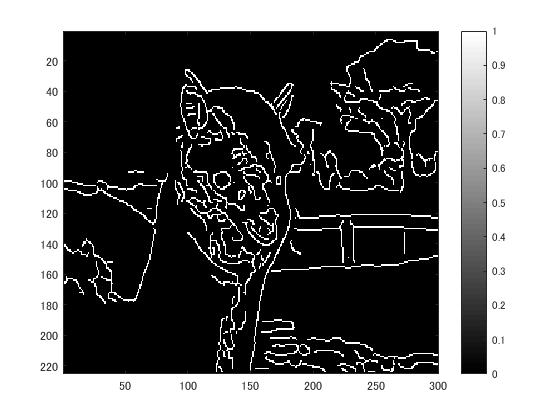
\includegraphics[width=10cm]{8-3.jpg}
 \end{center}
 \caption{エッジの抽出(キャニー法)}
\end{figure}

\section{考察}
画像のエッジの抽出を行った、キャニー法、ソベル法、プレウィット法の順にエッジの抽出が細かくできることが分かった。
\end{document}